\documentclass{article} % For LaTeX2e
\usepackage{iclr2019_conference,times}

% Optional math commands from https://github.com/goodfeli/dlbook_notation.
%%%%% NEW MATH DEFINITIONS %%%%%

\usepackage{amsmath,amsfonts,bm}

% Mark sections of captions for referring to divisions of figures
\newcommand{\figleft}{{\em (Left)}}
\newcommand{\figcenter}{{\em (Center)}}
\newcommand{\figright}{{\em (Right)}}
\newcommand{\figtop}{{\em (Top)}}
\newcommand{\figbottom}{{\em (Bottom)}}
\newcommand{\captiona}{{\em (a)}}
\newcommand{\captionb}{{\em (b)}}
\newcommand{\captionc}{{\em (c)}}
\newcommand{\captiond}{{\em (d)}}

% Highlight a newly defined term
\newcommand{\newterm}[1]{{\bf #1}}


% Figure reference, lower-case.
\def\figref#1{figure~\ref{#1}}
% Figure reference, capital. For start of sentence
\def\Figref#1{Figure~\ref{#1}}
\def\twofigref#1#2{figures \ref{#1} and \ref{#2}}
\def\quadfigref#1#2#3#4{figures \ref{#1}, \ref{#2}, \ref{#3} and \ref{#4}}
% Section reference, lower-case.
\def\secref#1{section~\ref{#1}}
% Section reference, capital.
\def\Secref#1{Section~\ref{#1}}
% Reference to two sections.
\def\twosecrefs#1#2{sections \ref{#1} and \ref{#2}}
% Reference to three sections.
\def\secrefs#1#2#3{sections \ref{#1}, \ref{#2} and \ref{#3}}
% Reference to an equation, lower-case.
\def\eqref#1{equation~\ref{#1}}
% Reference to an equation, upper case
\def\Eqref#1{Equation~\ref{#1}}
% A raw reference to an equation---avoid using if possible
\def\plaineqref#1{\ref{#1}}
% Reference to a chapter, lower-case.
\def\chapref#1{chapter~\ref{#1}}
% Reference to an equation, upper case.
\def\Chapref#1{Chapter~\ref{#1}}
% Reference to a range of chapters
\def\rangechapref#1#2{chapters\ref{#1}--\ref{#2}}
% Reference to an algorithm, lower-case.
\def\algref#1{algorithm~\ref{#1}}
% Reference to an algorithm, upper case.
\def\Algref#1{Algorithm~\ref{#1}}
\def\twoalgref#1#2{algorithms \ref{#1} and \ref{#2}}
\def\Twoalgref#1#2{Algorithms \ref{#1} and \ref{#2}}
% Reference to a part, lower case
\def\partref#1{part~\ref{#1}}
% Reference to a part, upper case
\def\Partref#1{Part~\ref{#1}}
\def\twopartref#1#2{parts \ref{#1} and \ref{#2}}

\def\ceil#1{\lceil #1 \rceil}
\def\floor#1{\lfloor #1 \rfloor}
\def\1{\bm{1}}
\newcommand{\train}{\mathcal{D}}
\newcommand{\valid}{\mathcal{D_{\mathrm{valid}}}}
\newcommand{\test}{\mathcal{D_{\mathrm{test}}}}

\def\eps{{\epsilon}}


% Random variables
\def\reta{{\textnormal{$\eta$}}}
\def\ra{{\textnormal{a}}}
\def\rb{{\textnormal{b}}}
\def\rc{{\textnormal{c}}}
\def\rd{{\textnormal{d}}}
\def\re{{\textnormal{e}}}
\def\rf{{\textnormal{f}}}
\def\rg{{\textnormal{g}}}
\def\rh{{\textnormal{h}}}
\def\ri{{\textnormal{i}}}
\def\rj{{\textnormal{j}}}
\def\rk{{\textnormal{k}}}
\def\rl{{\textnormal{l}}}
% rm is already a command, just don't name any random variables m
\def\rn{{\textnormal{n}}}
\def\ro{{\textnormal{o}}}
\def\rp{{\textnormal{p}}}
\def\rq{{\textnormal{q}}}
\def\rr{{\textnormal{r}}}
\def\rs{{\textnormal{s}}}
\def\rt{{\textnormal{t}}}
\def\ru{{\textnormal{u}}}
\def\rv{{\textnormal{v}}}
\def\rw{{\textnormal{w}}}
\def\rx{{\textnormal{x}}}
\def\ry{{\textnormal{y}}}
\def\rz{{\textnormal{z}}}

% Random vectors
\def\rvepsilon{{\mathbf{\epsilon}}}
\def\rvtheta{{\mathbf{\theta}}}
\def\rva{{\mathbf{a}}}
\def\rvb{{\mathbf{b}}}
\def\rvc{{\mathbf{c}}}
\def\rvd{{\mathbf{d}}}
\def\rve{{\mathbf{e}}}
\def\rvf{{\mathbf{f}}}
\def\rvg{{\mathbf{g}}}
\def\rvh{{\mathbf{h}}}
\def\rvu{{\mathbf{i}}}
\def\rvj{{\mathbf{j}}}
\def\rvk{{\mathbf{k}}}
\def\rvl{{\mathbf{l}}}
\def\rvm{{\mathbf{m}}}
\def\rvn{{\mathbf{n}}}
\def\rvo{{\mathbf{o}}}
\def\rvp{{\mathbf{p}}}
\def\rvq{{\mathbf{q}}}
\def\rvr{{\mathbf{r}}}
\def\rvs{{\mathbf{s}}}
\def\rvt{{\mathbf{t}}}
\def\rvu{{\mathbf{u}}}
\def\rvv{{\mathbf{v}}}
\def\rvw{{\mathbf{w}}}
\def\rvx{{\mathbf{x}}}
\def\rvy{{\mathbf{y}}}
\def\rvz{{\mathbf{z}}}

% Elements of random vectors
\def\erva{{\textnormal{a}}}
\def\ervb{{\textnormal{b}}}
\def\ervc{{\textnormal{c}}}
\def\ervd{{\textnormal{d}}}
\def\erve{{\textnormal{e}}}
\def\ervf{{\textnormal{f}}}
\def\ervg{{\textnormal{g}}}
\def\ervh{{\textnormal{h}}}
\def\ervi{{\textnormal{i}}}
\def\ervj{{\textnormal{j}}}
\def\ervk{{\textnormal{k}}}
\def\ervl{{\textnormal{l}}}
\def\ervm{{\textnormal{m}}}
\def\ervn{{\textnormal{n}}}
\def\ervo{{\textnormal{o}}}
\def\ervp{{\textnormal{p}}}
\def\ervq{{\textnormal{q}}}
\def\ervr{{\textnormal{r}}}
\def\ervs{{\textnormal{s}}}
\def\ervt{{\textnormal{t}}}
\def\ervu{{\textnormal{u}}}
\def\ervv{{\textnormal{v}}}
\def\ervw{{\textnormal{w}}}
\def\ervx{{\textnormal{x}}}
\def\ervy{{\textnormal{y}}}
\def\ervz{{\textnormal{z}}}

% Random matrices
\def\rmA{{\mathbf{A}}}
\def\rmB{{\mathbf{B}}}
\def\rmC{{\mathbf{C}}}
\def\rmD{{\mathbf{D}}}
\def\rmE{{\mathbf{E}}}
\def\rmF{{\mathbf{F}}}
\def\rmG{{\mathbf{G}}}
\def\rmH{{\mathbf{H}}}
\def\rmI{{\mathbf{I}}}
\def\rmJ{{\mathbf{J}}}
\def\rmK{{\mathbf{K}}}
\def\rmL{{\mathbf{L}}}
\def\rmM{{\mathbf{M}}}
\def\rmN{{\mathbf{N}}}
\def\rmO{{\mathbf{O}}}
\def\rmP{{\mathbf{P}}}
\def\rmQ{{\mathbf{Q}}}
\def\rmR{{\mathbf{R}}}
\def\rmS{{\mathbf{S}}}
\def\rmT{{\mathbf{T}}}
\def\rmU{{\mathbf{U}}}
\def\rmV{{\mathbf{V}}}
\def\rmW{{\mathbf{W}}}
\def\rmX{{\mathbf{X}}}
\def\rmY{{\mathbf{Y}}}
\def\rmZ{{\mathbf{Z}}}

% Elements of random matrices
\def\ermA{{\textnormal{A}}}
\def\ermB{{\textnormal{B}}}
\def\ermC{{\textnormal{C}}}
\def\ermD{{\textnormal{D}}}
\def\ermE{{\textnormal{E}}}
\def\ermF{{\textnormal{F}}}
\def\ermG{{\textnormal{G}}}
\def\ermH{{\textnormal{H}}}
\def\ermI{{\textnormal{I}}}
\def\ermJ{{\textnormal{J}}}
\def\ermK{{\textnormal{K}}}
\def\ermL{{\textnormal{L}}}
\def\ermM{{\textnormal{M}}}
\def\ermN{{\textnormal{N}}}
\def\ermO{{\textnormal{O}}}
\def\ermP{{\textnormal{P}}}
\def\ermQ{{\textnormal{Q}}}
\def\ermR{{\textnormal{R}}}
\def\ermS{{\textnormal{S}}}
\def\ermT{{\textnormal{T}}}
\def\ermU{{\textnormal{U}}}
\def\ermV{{\textnormal{V}}}
\def\ermW{{\textnormal{W}}}
\def\ermX{{\textnormal{X}}}
\def\ermY{{\textnormal{Y}}}
\def\ermZ{{\textnormal{Z}}}

% Vectors
\def\vzero{{\bm{0}}}
\def\vone{{\bm{1}}}
\def\vmu{{\bm{\mu}}}
\def\vtheta{{\bm{\theta}}}
\def\va{{\bm{a}}}
\def\vb{{\bm{b}}}
\def\vc{{\bm{c}}}
\def\vd{{\bm{d}}}
\def\ve{{\bm{e}}}
\def\vf{{\bm{f}}}
\def\vg{{\bm{g}}}
\def\vh{{\bm{h}}}
\def\vi{{\bm{i}}}
\def\vj{{\bm{j}}}
\def\vk{{\bm{k}}}
\def\vl{{\bm{l}}}
\def\vm{{\bm{m}}}
\def\vn{{\bm{n}}}
\def\vo{{\bm{o}}}
\def\vp{{\bm{p}}}
\def\vq{{\bm{q}}}
\def\vr{{\bm{r}}}
\def\vs{{\bm{s}}}
\def\vt{{\bm{t}}}
\def\vu{{\bm{u}}}
\def\vv{{\bm{v}}}
\def\vw{{\bm{w}}}
\def\vx{{\bm{x}}}
\def\vy{{\bm{y}}}
\def\vz{{\bm{z}}}

% Elements of vectors
\def\evalpha{{\alpha}}
\def\evbeta{{\beta}}
\def\evepsilon{{\epsilon}}
\def\evlambda{{\lambda}}
\def\evomega{{\omega}}
\def\evmu{{\mu}}
\def\evpsi{{\psi}}
\def\evsigma{{\sigma}}
\def\evtheta{{\theta}}
\def\eva{{a}}
\def\evb{{b}}
\def\evc{{c}}
\def\evd{{d}}
\def\eve{{e}}
\def\evf{{f}}
\def\evg{{g}}
\def\evh{{h}}
\def\evi{{i}}
\def\evj{{j}}
\def\evk{{k}}
\def\evl{{l}}
\def\evm{{m}}
\def\evn{{n}}
\def\evo{{o}}
\def\evp{{p}}
\def\evq{{q}}
\def\evr{{r}}
\def\evs{{s}}
\def\evt{{t}}
\def\evu{{u}}
\def\evv{{v}}
\def\evw{{w}}
\def\evx{{x}}
\def\evy{{y}}
\def\evz{{z}}

% Matrix
\def\mA{{\bm{A}}}
\def\mB{{\bm{B}}}
\def\mC{{\bm{C}}}
\def\mD{{\bm{D}}}
\def\mE{{\bm{E}}}
\def\mF{{\bm{F}}}
\def\mG{{\bm{G}}}
\def\mH{{\bm{H}}}
\def\mI{{\bm{I}}}
\def\mJ{{\bm{J}}}
\def\mK{{\bm{K}}}
\def\mL{{\bm{L}}}
\def\mM{{\bm{M}}}
\def\mN{{\bm{N}}}
\def\mO{{\bm{O}}}
\def\mP{{\bm{P}}}
\def\mQ{{\bm{Q}}}
\def\mR{{\bm{R}}}
\def\mS{{\bm{S}}}
\def\mT{{\bm{T}}}
\def\mU{{\bm{U}}}
\def\mV{{\bm{V}}}
\def\mW{{\bm{W}}}
\def\mX{{\bm{X}}}
\def\mY{{\bm{Y}}}
\def\mZ{{\bm{Z}}}
\def\mBeta{{\bm{\beta}}}
\def\mPhi{{\bm{\Phi}}}
\def\mLambda{{\bm{\Lambda}}}
\def\mSigma{{\bm{\Sigma}}}

% Tensor
\DeclareMathAlphabet{\mathsfit}{\encodingdefault}{\sfdefault}{m}{sl}
\SetMathAlphabet{\mathsfit}{bold}{\encodingdefault}{\sfdefault}{bx}{n}
\newcommand{\tens}[1]{\bm{\mathsfit{#1}}}
\def\tA{{\tens{A}}}
\def\tB{{\tens{B}}}
\def\tC{{\tens{C}}}
\def\tD{{\tens{D}}}
\def\tE{{\tens{E}}}
\def\tF{{\tens{F}}}
\def\tG{{\tens{G}}}
\def\tH{{\tens{H}}}
\def\tI{{\tens{I}}}
\def\tJ{{\tens{J}}}
\def\tK{{\tens{K}}}
\def\tL{{\tens{L}}}
\def\tM{{\tens{M}}}
\def\tN{{\tens{N}}}
\def\tO{{\tens{O}}}
\def\tP{{\tens{P}}}
\def\tQ{{\tens{Q}}}
\def\tR{{\tens{R}}}
\def\tS{{\tens{S}}}
\def\tT{{\tens{T}}}
\def\tU{{\tens{U}}}
\def\tV{{\tens{V}}}
\def\tW{{\tens{W}}}
\def\tX{{\tens{X}}}
\def\tY{{\tens{Y}}}
\def\tZ{{\tens{Z}}}


% Graph
\def\gA{{\mathcal{A}}}
\def\gB{{\mathcal{B}}}
\def\gC{{\mathcal{C}}}
\def\gD{{\mathcal{D}}}
\def\gE{{\mathcal{E}}}
\def\gF{{\mathcal{F}}}
\def\gG{{\mathcal{G}}}
\def\gH{{\mathcal{H}}}
\def\gI{{\mathcal{I}}}
\def\gJ{{\mathcal{J}}}
\def\gK{{\mathcal{K}}}
\def\gL{{\mathcal{L}}}
\def\gM{{\mathcal{M}}}
\def\gN{{\mathcal{N}}}
\def\gO{{\mathcal{O}}}
\def\gP{{\mathcal{P}}}
\def\gQ{{\mathcal{Q}}}
\def\gR{{\mathcal{R}}}
\def\gS{{\mathcal{S}}}
\def\gT{{\mathcal{T}}}
\def\gU{{\mathcal{U}}}
\def\gV{{\mathcal{V}}}
\def\gW{{\mathcal{W}}}
\def\gX{{\mathcal{X}}}
\def\gY{{\mathcal{Y}}}
\def\gZ{{\mathcal{Z}}}

% Sets
\def\sA{{\mathbb{A}}}
\def\sB{{\mathbb{B}}}
\def\sC{{\mathbb{C}}}
\def\sD{{\mathbb{D}}}
% Don't use a set called E, because this would be the same as our symbol
% for expectation.
\def\sF{{\mathbb{F}}}
\def\sG{{\mathbb{G}}}
\def\sH{{\mathbb{H}}}
\def\sI{{\mathbb{I}}}
\def\sJ{{\mathbb{J}}}
\def\sK{{\mathbb{K}}}
\def\sL{{\mathbb{L}}}
\def\sM{{\mathbb{M}}}
\def\sN{{\mathbb{N}}}
\def\sO{{\mathbb{O}}}
\def\sP{{\mathbb{P}}}
\def\sQ{{\mathbb{Q}}}
\def\sR{{\mathbb{R}}}
\def\sS{{\mathbb{S}}}
\def\sT{{\mathbb{T}}}
\def\sU{{\mathbb{U}}}
\def\sV{{\mathbb{V}}}
\def\sW{{\mathbb{W}}}
\def\sX{{\mathbb{X}}}
\def\sY{{\mathbb{Y}}}
\def\sZ{{\mathbb{Z}}}

% Entries of a matrix
\def\emLambda{{\Lambda}}
\def\emA{{A}}
\def\emB{{B}}
\def\emC{{C}}
\def\emD{{D}}
\def\emE{{E}}
\def\emF{{F}}
\def\emG{{G}}
\def\emH{{H}}
\def\emI{{I}}
\def\emJ{{J}}
\def\emK{{K}}
\def\emL{{L}}
\def\emM{{M}}
\def\emN{{N}}
\def\emO{{O}}
\def\emP{{P}}
\def\emQ{{Q}}
\def\emR{{R}}
\def\emS{{S}}
\def\emT{{T}}
\def\emU{{U}}
\def\emV{{V}}
\def\emW{{W}}
\def\emX{{X}}
\def\emY{{Y}}
\def\emZ{{Z}}
\def\emSigma{{\Sigma}}

% entries of a tensor
% Same font as tensor, without \bm wrapper
\newcommand{\etens}[1]{\mathsfit{#1}}
\def\etLambda{{\etens{\Lambda}}}
\def\etA{{\etens{A}}}
\def\etB{{\etens{B}}}
\def\etC{{\etens{C}}}
\def\etD{{\etens{D}}}
\def\etE{{\etens{E}}}
\def\etF{{\etens{F}}}
\def\etG{{\etens{G}}}
\def\etH{{\etens{H}}}
\def\etI{{\etens{I}}}
\def\etJ{{\etens{J}}}
\def\etK{{\etens{K}}}
\def\etL{{\etens{L}}}
\def\etM{{\etens{M}}}
\def\etN{{\etens{N}}}
\def\etO{{\etens{O}}}
\def\etP{{\etens{P}}}
\def\etQ{{\etens{Q}}}
\def\etR{{\etens{R}}}
\def\etS{{\etens{S}}}
\def\etT{{\etens{T}}}
\def\etU{{\etens{U}}}
\def\etV{{\etens{V}}}
\def\etW{{\etens{W}}}
\def\etX{{\etens{X}}}
\def\etY{{\etens{Y}}}
\def\etZ{{\etens{Z}}}

% The true underlying data generating distribution
\newcommand{\pdata}{p_{\rm{data}}}
% The empirical distribution defined by the training set
\newcommand{\ptrain}{\hat{p}_{\rm{data}}}
\newcommand{\Ptrain}{\hat{P}_{\rm{data}}}
% The model distribution
\newcommand{\pmodel}{p_{\rm{model}}}
\newcommand{\Pmodel}{P_{\rm{model}}}
\newcommand{\ptildemodel}{\tilde{p}_{\rm{model}}}
% Stochastic autoencoder distributions
\newcommand{\pencode}{p_{\rm{encoder}}}
\newcommand{\pdecode}{p_{\rm{decoder}}}
\newcommand{\precons}{p_{\rm{reconstruct}}}

\newcommand{\laplace}{\mathrm{Laplace}} % Laplace distribution

\newcommand{\E}{\mathbb{E}}
\newcommand{\Ls}{\mathcal{L}}
\newcommand{\R}{\mathbb{R}}
\newcommand{\emp}{\tilde{p}}
\newcommand{\lr}{\alpha}
\newcommand{\reg}{\lambda}
\newcommand{\rect}{\mathrm{rectifier}}
\newcommand{\softmax}{\mathrm{softmax}}
\newcommand{\sigmoid}{\sigma}
\newcommand{\softplus}{\zeta}
\newcommand{\KL}{D_{\mathrm{KL}}}
\newcommand{\Var}{\mathrm{Var}}
\newcommand{\standarderror}{\mathrm{SE}}
\newcommand{\Cov}{\mathrm{Cov}}
% Wolfram Mathworld says $L^2$ is for function spaces and $\ell^2$ is for vectors
% But then they seem to use $L^2$ for vectors throughout the site, and so does
% wikipedia.
\newcommand{\normlzero}{L^0}
\newcommand{\normlone}{L^1}
\newcommand{\normltwo}{L^2}
\newcommand{\normlp}{L^p}
\newcommand{\normmax}{L^\infty}

\newcommand{\parents}{Pa} % See usage in notation.tex. Chosen to match Daphne's book.

\DeclareMathOperator*{\argmax}{arg\,max}
\DeclareMathOperator*{\argmin}{arg\,min}

\DeclareMathOperator{\sign}{sign}
\DeclareMathOperator{\Tr}{Tr}
\let\ab\allowbreak


\usepackage{hyperref}
\usepackage{url}
\usepackage{graphicx}

\title{A reproduce report of paper: \\ 
ImageNet-trained CNNs are biased towards texture; increasing shape bias improves accuracy and robustness}

% Authors must not appear in the submitted version. They should be hidden
% as long as the \iclrfinalcopy macro remains commented out below.
% Non-anonymous submissions will be rejected without review.

\author{Shaobo Xu* \& Peihao Ren*  \\
School of Electronics and Computer Science\\
University of Southampton\\
Southampton, SO17 1BJ, United Kingdom\\
\texttt{\{sx2n18, pr1y18\}@soton.ac.uk} \\
}

% The \author macro works with any number of authors. There are two commands
% used to separate the names and addresses of multiple authors: \And and \AND.
%
% Using \And between authors leaves it to \LaTeX{} to determine where to break
% the lines. Using \AND forces a linebreak at that point. So, if \LaTeX{}
% puts 3 of 4 authors names on the first line, and the last on the second
% line, try using \AND instead of \And before the third author name.

\newcommand{\fix}{\marginpar{FIX}}
\newcommand{\new}{\marginpar{NEW}}

\iclrfinalcopy % Uncomment for camera-ready version, but NOT for submission.
\begin{document}


\maketitle

\begin{abstract}

We reproduced an oral ICLR paper, named ``ImageNet-trained CNNs are biased towards texture; increasing shape bias improves accuracy and robustness''. We implemented the most important part in the original paper and briefly discussed  experiments on a subset of the ImageNet dataset (only 16 classes). 
We found that ResNet-50 trained on Stylized ImageNet is more accurate and robust than the same network trained only on ImageNet. We also verified that shape-based representations are more robust than the texture representations.
All codes except the style transfer part are written by the two authors.

\end{abstract}

\section{Introduction}

Ever since AlexNet~\cite{krizhevsky2012imagenet} won the competition, deep neural networks (DNN) becomes a more and more hot topics in the image-relevant field. However, the author of the paper "ImageNet-trained CNNs are biased towards texture; increasing shape bias improves accuracy and robustness" has found that the popular DNN structures are actually biased towards texture which stands opposite to human behaviour. The author of the original paper has proposed one way to eliminate or partially eliminate the bias, that is by training the NN model on the stylized dataset. 

\section{Data}

\subsection{16-classes ImageNet dataset}
We downloaded the famous ImageNet dataset~\cite{deng2009imagenet}. It contains 1000 classes of images and each of the classes has about 1000 pictures. This data set is too big for us, thus we choose 16 classes of them as listed in the paper. The 16 classes are knife, keyboard, elephant, bicycle, airplane, clock, oven, chair, bear, boat, cat, bottle, truck, car, bird, dog. Each of these classes has 1300 pictures which is still too big since we would introduce stylized images in the following section which multiply the number of images by 8.

Hence our final data structure contains a training set and a validation set. Each set has 16 classes of different types of images. The training set has 400 images in each class while the validation set has 100 images in each class.

\subsection{Stylized Image}

As is done in the original paper, the input images are stylized. We use the algorithm from GitHub (https://github.com/rgeirhos/Stylized-ImageNet) to transfer our original image input to several different styles. This stylizing method is from \cite{huang2017arbitrary}. It uses the pictures from  Kaggle's painter-by-numbers dataset (https://www.kaggle.com/c/painter-by-numbers/data) as style pictures, then use an encoder to get the representation of the style picture and the original picture. The data is then fed to an Adaptive Instance Normalization (AdaIN) layer and a decoder. The final stylized picture is given by the original picture and the data from the decoder.

\begin{figure}[!h]
\centering{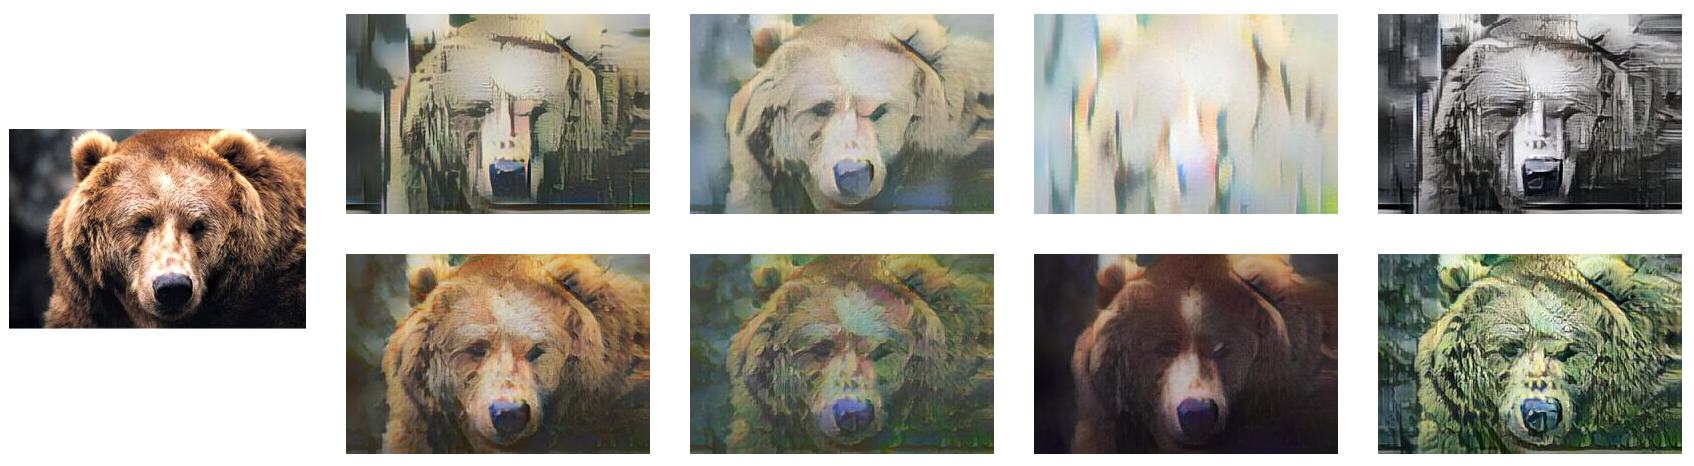
\includegraphics[width=0.96\textwidth]{img/bear}}
\caption{Example output of the stylized image. For each input image, we put it into the stylizing algorithm and then got 8 output images with random styles.}
\label{bear}
\end{figure}

The stylized images are shown in figure~\ref{bear}. Human can easily find that these 8 stylized images are from a same original image. That is because we focus on the shape of the bear in stead of its texture. 

In this report paper, we use IN to represent 16 classes ImageNet, and use SIN to represent Stylized 16 classes ImageNet.

\section{Experiment}

\subsection{training convergence}

Since our dataset is different from the original paper, we plot the accuracy curve during each epoch in order to show the convergence performance on our dataset.

\begin{figure}[!h]
\centering{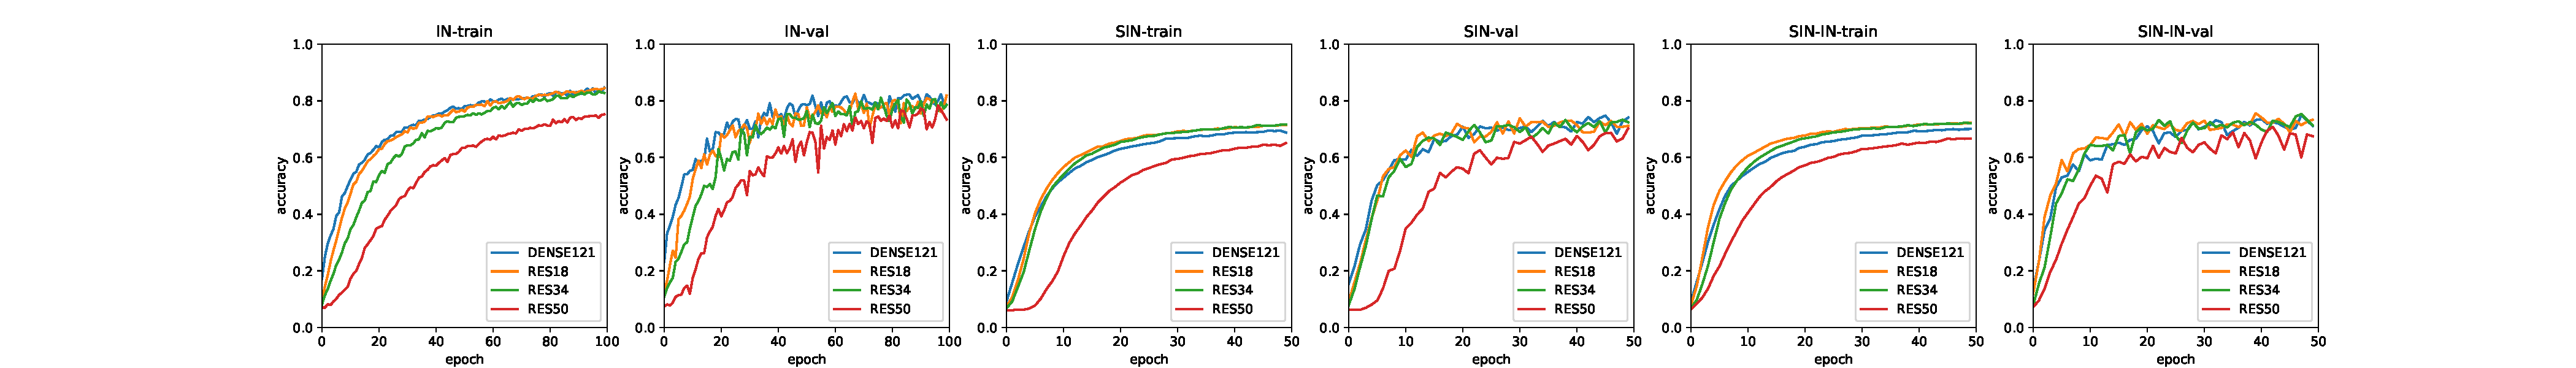
\includegraphics[width=0.98\textwidth]{img/converge}}
\caption{Top 1 accuracy on different datasets. In the figure above, IN train represents the top 1 training accuracy on IN dateset and SIN represents the top 1 accuracy on SIN dataset.}
\label{converge}
\end{figure}

The results of our loss and accuracy curve on different datasets are shown in Figure~\ref{converge}. Our dataset only contains 8000 images (6400 for training and 1600 for validation). This means a complex DNN may cause overfitting thus leads to the situation that a simple DNN may get better performance than a complex DNN.

On the ImageNet dataset, we trained the model for 100 epochs while on the SIN dataset and the SIN+IN dataset, we trained the model for 50 epochs. This is because we need to get the converged accuracy of each model. IN is too small that needs more epochs to converge. SIN, on the other hand, is 8 times as large as IN, thus needs much less epochs to converge. Other parameters are the same as that in the original paper.

\subsection{texture shape bias}

The key point of the reproduced paper is, the DNNs which were trained on ImageNet, are biased towards texture. Hence the author of the original paper did the an experiment to show this bias.

\begin{table}[!h]
\caption{Top 1 and top 5 accuracy of different neural networks training on different datasets. We trained different neural networks on different datasets and evaluated them on these datasets. The number of training epochs we choose are, IN:100, SIN:50.}
\label{sample-table}
\begin{center}
\begin{tabular}{l c c c c}
\bf Model & $\textbf{IN} \to \textbf{IN}$  & $\textbf{IN} \to \textbf{SIN}$  & $\textbf{SIN} \to \textbf{SIN}$  & $\textbf{SIN}\to\textbf{IN}$ \\
\hline \\  
ResNet-18    &{\bf82.6} / 96.9   &27.3 / 62.4  &73.8 / 94.1   &78.8 / 95.6\\
ResNet-34    &81.1 / 96.8   &28.3 / 62.2   &73.3 / 93.6    & 79.3 / 94.8\\
ResNet-50   &78.4 / 95.8   &20.9 / 54.6   &70.3 / 92.3   &77.5 / 94.7\\
DenseNet-121   & 82.2 / {\bf97.0}   &25.0 / 58.9   &74.8 / 94.2   &\bf79.6 / 95.8\\
\end{tabular}
\label{original}
\end{center}
\end{table}

Table~\ref{original} shows our results on the experience. In this experiment, we trained 4 different DNNs on different datasets, and evaluated them on different datasets as the author of the original paper did. We used the DenseNet~\cite{huang2017densely} instead of the BagNet as the author of the original paper did because the BagNet has many large convolution kernels which needs long time and large memory to train.

The results in the table show that DenseNet-121 outperforms than every ResNet in all datasets. The models trained on IN have poor performance on SIN while the models trained on SIN have much better performance on IN. This may be a prove to the author's opinion that ImageNet trained models are biased towards texture since the texture of SIN and IN are almost totally different.

\subsection{improve dnn towards shape}

The next experiment we did is to show that the SIN dataset can make the original DNN pay more attention to the shape of the input image.

\begin{table}[!h]
\caption{Results of RestNet 50 training on different training data. The parameters are set the same as that in the former subsection. The fine-tune part is trained on the IN dataset with 50 epochs.}
\label{sample-table}
\begin{center}
\begin{tabular}{l c c c }
\bf training set & \bf fine-tune & \bf top 1 acc  & \bf top 5 acc
\\ \hline \\
IN   & - &78.4   &95.8 \\
SIN  & -   &77.5   &94.8 \\
SIN+IN   & -   &78.8   &95.6 \\
SIN+IN   & IN   & \bf 89.0   & \bf 97.9 \\
\end{tabular}
\label{improved}
\end{center}
\end{table}

Table~\ref{improved} clearly shows that using SIN+IN and fine-tune will improve the original model. As is shown in the table, if we train the ResNet-50 model on SIN+IN dataset, and then use IN to fine tune it, we got a better accuracy result than the results of all original networks on IN in the former subsection.


\subsection{robustness} 

We also tested the robustness of the models. As it is proposed in the original paper, we tried to add several distortions to the validation set, including adding noises, changing the contrast and blurring. We added uniform noise and Gaussian noise with different amplitudes. 

\begin{figure}[!h]
\centering{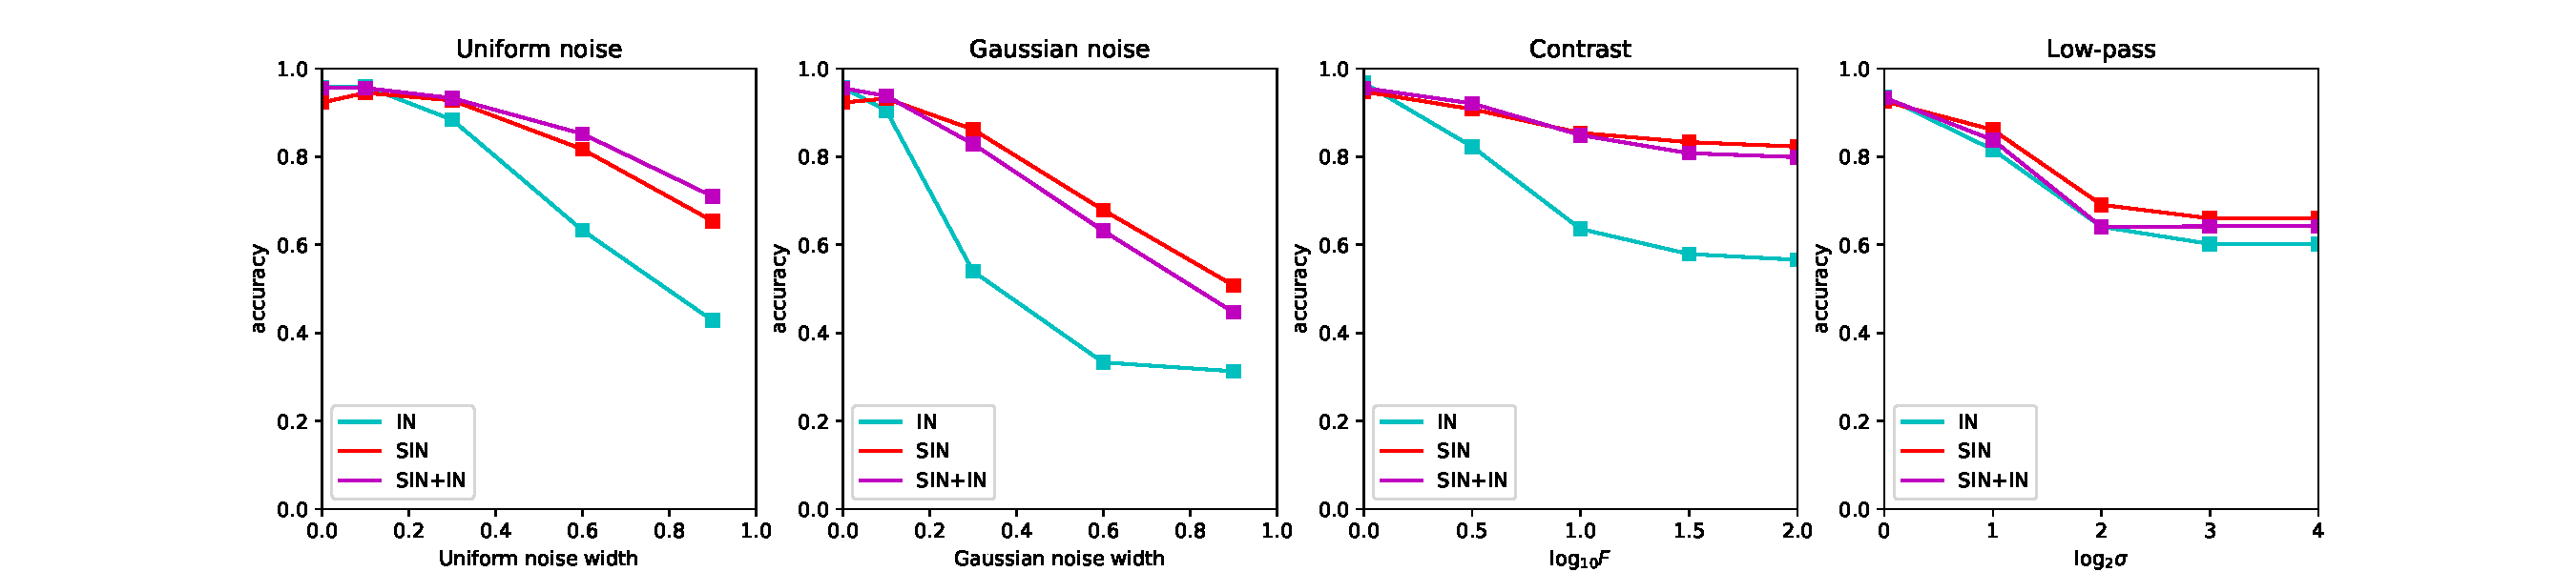
\includegraphics[width=0.96\textwidth]{img/noise}}
\caption{Top 5 accuracy on distorted images in validation set. ResNet-50 trained on SIN is more robust towards distortions than the same network trained on IN.}
\label{noise}
\end{figure}



We blurred images using low-pass Gaussian filter with a fixed kernel size ($N=15$) and different variance $\sigma$.

We can conclude from figure~\ref{noise} that the ResNet-50 model trained on the original IN dataset is the least robust model. It performs the worst when getting any noise. However, the model trained on SIN and SIN+IN has similar performance. This means that training on the SIN dataset do have a positive effect on robustness.

\section{Discussion}

The original paper contains many psychophysical experiments which are hard to reproduce. Also, training on such a large dataset (9 times ImageNet size for SIN+IN dataset) is almost impossible for our computing resources. Hence we need to weaken some of the experiments and focus on the important experiments which give the main idea of the author. But even we use the 16 classes ImageNet, it still needs about 2.5 minutes to train a single epoch on the SIN dataset. This means the computing time is another handicap in our experiments.

The method proposed by the original paper's author is essentially a data augmentation method. It can more or less eliminate the bias towards texture and improve the accuracy a little bit. However, the most important idea of the original paper is that we can use a stylized dataset as a complementary dataset of the original one. This is a new perspective of improve the networks since we used to change the structure of the model in order to get better performance.


\section{Conclusion}

In this report, we have successfully reproduced most important parts of the original paper and has proved the author's idea that the models trained on ImageNet is biased towards texture rather than shape. We've also proved that training on SIN or SIN+IN and fine-tuning on IN will eliminate this bias to some extent. This paper warns us that we should build dataset that has less bias towards texture since this is the way we humans behave. Or the model we trained may have poor generalization performance.



\subsubsection*{Acknowledgments}

We would like to thank Dr.Jonathon Hare and Dr.Kate Farrahi for delivering the Differentiable Programming (and Deep Learning) module. The deep learning module and this reproducibility challenge is challenging but very meaningful. During reproducing the original paper, we've read a lot and learnt a lot about the state-of-the-art technologies in the deep learning field.

\bibliography{DL_reproduce}
\bibliographystyle{iclr2019_conference}

\end{document}
